\PassOptionsToPackage{unicode}{hyperref}
\documentclass[aspectratio=1610, professionalfonts, 9pt, t]{beamer}

\usefonttheme[onlymath]{serif}
\usetheme[showtotalframes]{tudo}


\usepackage{polyglossia}
\setmainlanguage{english}

% Mathematik
\usepackage{multicol}
\usepackage{graphicx}
\usepackage{amssymb}
\usepackage{amsmath}
\usepackage{mathtools}
\usepackage[
  math-style=ISO,
  bold-style=ISO,
  sans-style=italic,
  nabla=upright,
  partial=upright,
]{unicode-math}
\setmathfont{Latin Modern Math}
\usepackage{xparse}
\usepackage{braket}
\usepackage{ulem}
\usepackage{units}
\usepackage[locale=DE,separate-uncertainty=true,per-mode=reciprocal,output-decimal-marker={,},]{siunitx}
\usepackage[section]{placeins}
\usepackage{pdflscape}
\usepackage{expl3}
\usepackage{bookmark}
%Komma als Dezimaltrenner in der mathe Umgebung, um in Umgebungen wie [0, 2] ein Leerzeichen nach dem Komma zu erhalten einfach eins setzen
\usepackage{icomma}
\usepackage{cancel}
\usepackage{tikz}
\usepackage{feynman-tikz}
\usepackage{hyperref}
\usepackage{bookmark}
\usepackage{subfigure}
\usepackage{booktabs}

%%%%%%%%%%%%%%%%%%%%%%%%%%%%%%%%%%%%%%%%%%%%%%%%%%%%%%%%%%%%%%%%%%%%%%%%%%%%%%%%
%%%%%-------------Hier Titel/Autor/Grafik/Lehrstuhl eintragen--------------%%%%%
%%%%%%%%%%%%%%%%%%%%%%%%%%%%%%%%%%%%%%%%%%%%%%%%%%%%%%%%%%%%%%%%%%%%%%%%%%%%%%%%

%Titel:
\title{Kaonenexperimente im Wandel der Zeit}
%Autor
\author[F.~Koch]{Fabian Koch}
%Datum der Präsentation
\date{02.05.19}
%Lehrstuhl/Fakultät
\institute[Fakultät Physik ]{Fakultät Physik}

\begin{document}

\AtBeginSection[]
{
  \begin{frame}{Inhalt}
    \tableofcontents[currentsection]
  \end{frame}
}


\maketitle

\begin{frame}
  \frametitle{Übersicht}
  \tableofcontents
\end{frame}


\section{Was sind Kaonen}
  \begin{frame}{Was sind Kaonen?}
    \begin{columns}[onlytextwidth]
      \begin{column}{0.4\textwidth}
        \begin{figure}[ht]
          \begin{center}
            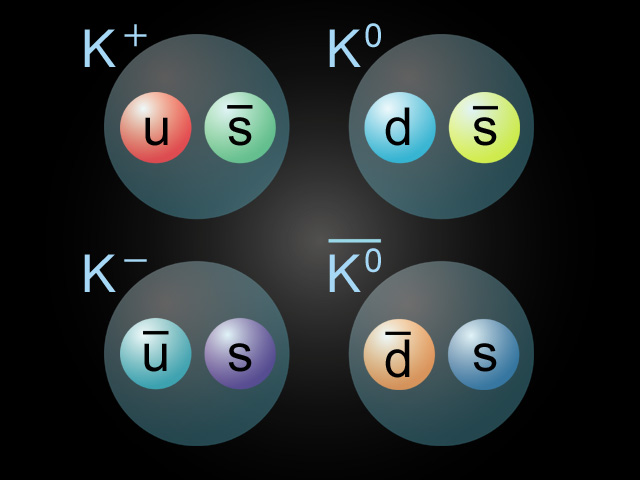
\includegraphics[height=0.6\textheight]{Images/Kaonen.png}
            \caption{Übersicht über die Kaonen}
          \end{center}
        \end{figure}
      \end{column}
      \begin{column}{0.5\textwidth}
        Kaonen:
        \begin{itemize}
          \item sind die leichtesten Teilchen mit Strangeness $S = \pm1$
          \item besitzen einen ganzzahligen Spin
          \item sind Bosonen
          \item verfügen über eine relativ lange Lebensdauer
        \end{itemize}
        \begin{table}
          \centering
          \begin{tabular}{
              S[table-format=6.0]
              S[table-format=3.5]
              @{${}\pm{}$}
              S[table-format=1.5]
              S[table-format=3.4]
              @{${}\pm{}$}
              S[table-format=1.4]
            }
              \toprule
              & \multicolumn{2}{c}{$m \:/\: \si{\mega\electronvolt}$} & \multicolumn{2}{c}{$\tau \:/\: 10^{-10} \si{\second}$} \\
              \midrule
              $K^{\pm}$   & 493.677 & 0.016 & 123.80 & 0.21 \\
              $K⁰_{S}$    & 497.614 & 0.024 & 0.8954 & 0.0004 \\
              $K⁰_{L}$    & 497.614 & 0.024 & 511.6  & 2.1 \\
              ${\pi}^{\pm}$ & 139.57018 & 0.00035 & 260.33 & 0.05 \\
              \bottomrule
          \end{tabular}
        \end{table}
      \end{column}
    \end{columns}
  \end{frame}

\section{Historische Kaonenexperimente}
  \begin{frame}{Weltkarte}
    %Hier könnte ihre Weltkarte stehen
  \end{frame}

\subsection{Entdeckung der Kaonen}
  \begin{frame}{Entdeckung der Kaonen}
    \begin{columns}[onlytextwidth]
      \begin{column}{0.4\textwidth}
        \begin{figure}[ht]
          \begin{center}
            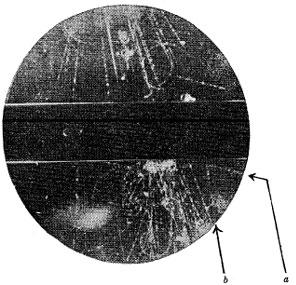
\includegraphics[height=0.6\textheight]{Images/Kaondiscovery.png}
            \caption{Nebelkammeraufnahme der kosmischen Höhenstrahlung von Rochester und Butler 1947}
          \end{center}
        \end{figure}
      \end{column}
      \begin{column}{0.5\textwidth}
        \begin{itemize}
          \item Entdeckung des ersten (neutralen) Kaons 1947 durch George Rochester et. al
          \item Höhenstrahlung wurde in Nebelkammer untersucht
          \item Zerfall eines neutralen Teilchens in ein positives und negatives Pion
          \begin{equation*}
            K^{0} \rightarrow \pi^{+} \pi^{-}
          \end{equation*}
          \item Entdeckung des positiv geladenen Kaons 1949 durch Powell in Kernreaktionen
          \item Zerfall eines positiven Kaons in zwei positive und ein negatives Pion
          \begin{equation*}
            K^{+} \rightarrow \pi^{+} \pi^{+} \pi^{-}
          \end{equation*}
        \end{itemize}
      \end{column}
    \end{columns}
  \end{frame}

  \begin{frame}{Seltsam lange Lebensdauer}
    \begin{columns}[onlytextwidth]
      \begin{column}{0.4\textwidth}
        \begin{figure}[ht]
          \begin{center}
            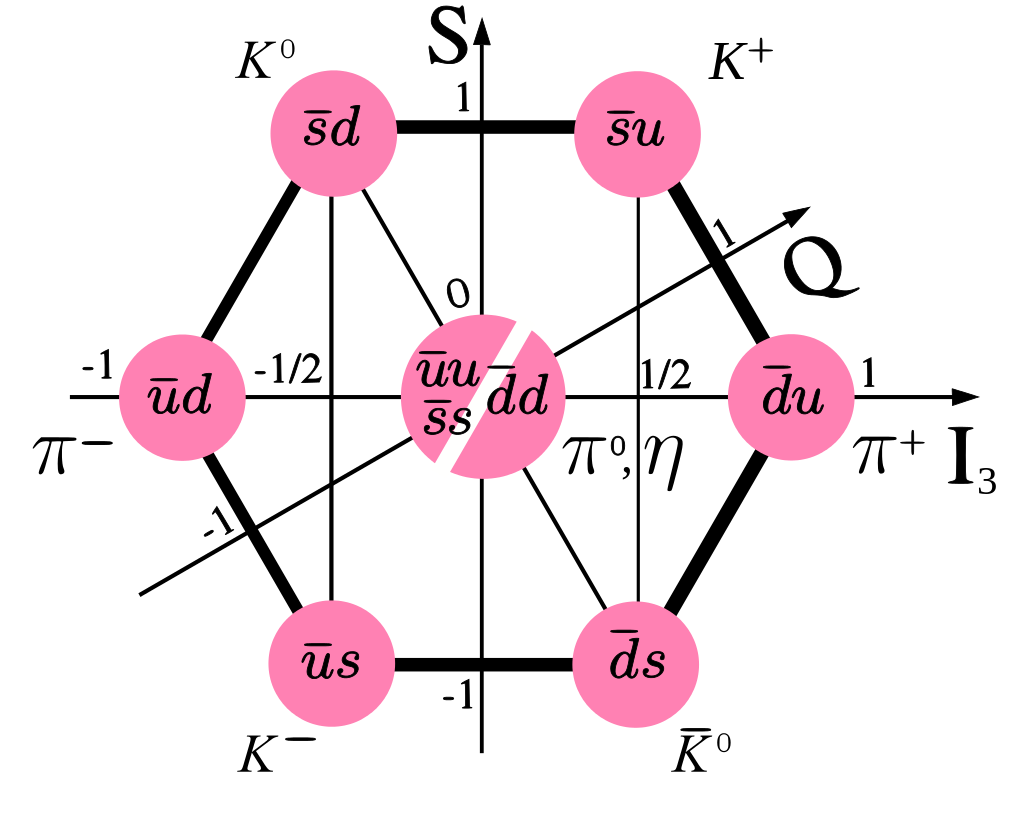
\includegraphics[height=0.6\textheight]{Images/Meson-octet.png} %Zuschnippeln
            \caption{Der achtfache Weg von Gell-Mann und Ne'eman}
          \end{center}
        \end{figure}
      \end{column}
      \begin{column}{0.5\textwidth}
        \begin{itemize}
          \item Konnten sehr leicht erzeugt werden (durch starke WW)
          \item Zerfielen aber sehr langsam $10^{-10}\si{\second}$ (durch schwache WW)
          \item Durch Gell-Mann 1953 Einführung einer neuen Teilcheneigenschaft/ Quantenzahl, der 'Strangeness' (der achtfache Weg)
          \item Kaonen sind leichteste Teilchen mit \textbf{S} $= \pm1$ und könnten somit nicht zerfallen, wenn \textbf{S} durch alle Kräfte erhalten wäre
          \item Einziger Zerfall somit über die flavourändernde schwache WW möglich
          \item \textbf{S} veranlasste Cabibo 1963 zur Postulierung des Cabibo-Winkels
        \end{itemize}
      \end{column}
    \end{columns}
  \end{frame}

\subsection{Paritätsverletzung}

  \begin{frame}{Paritätsverletzung und der Cosmotron}
    \begin{columns}[onlytextwidth]
      \begin{column}{0.4\textwidth}
        \begin{figure}[ht]
          \begin{center}
            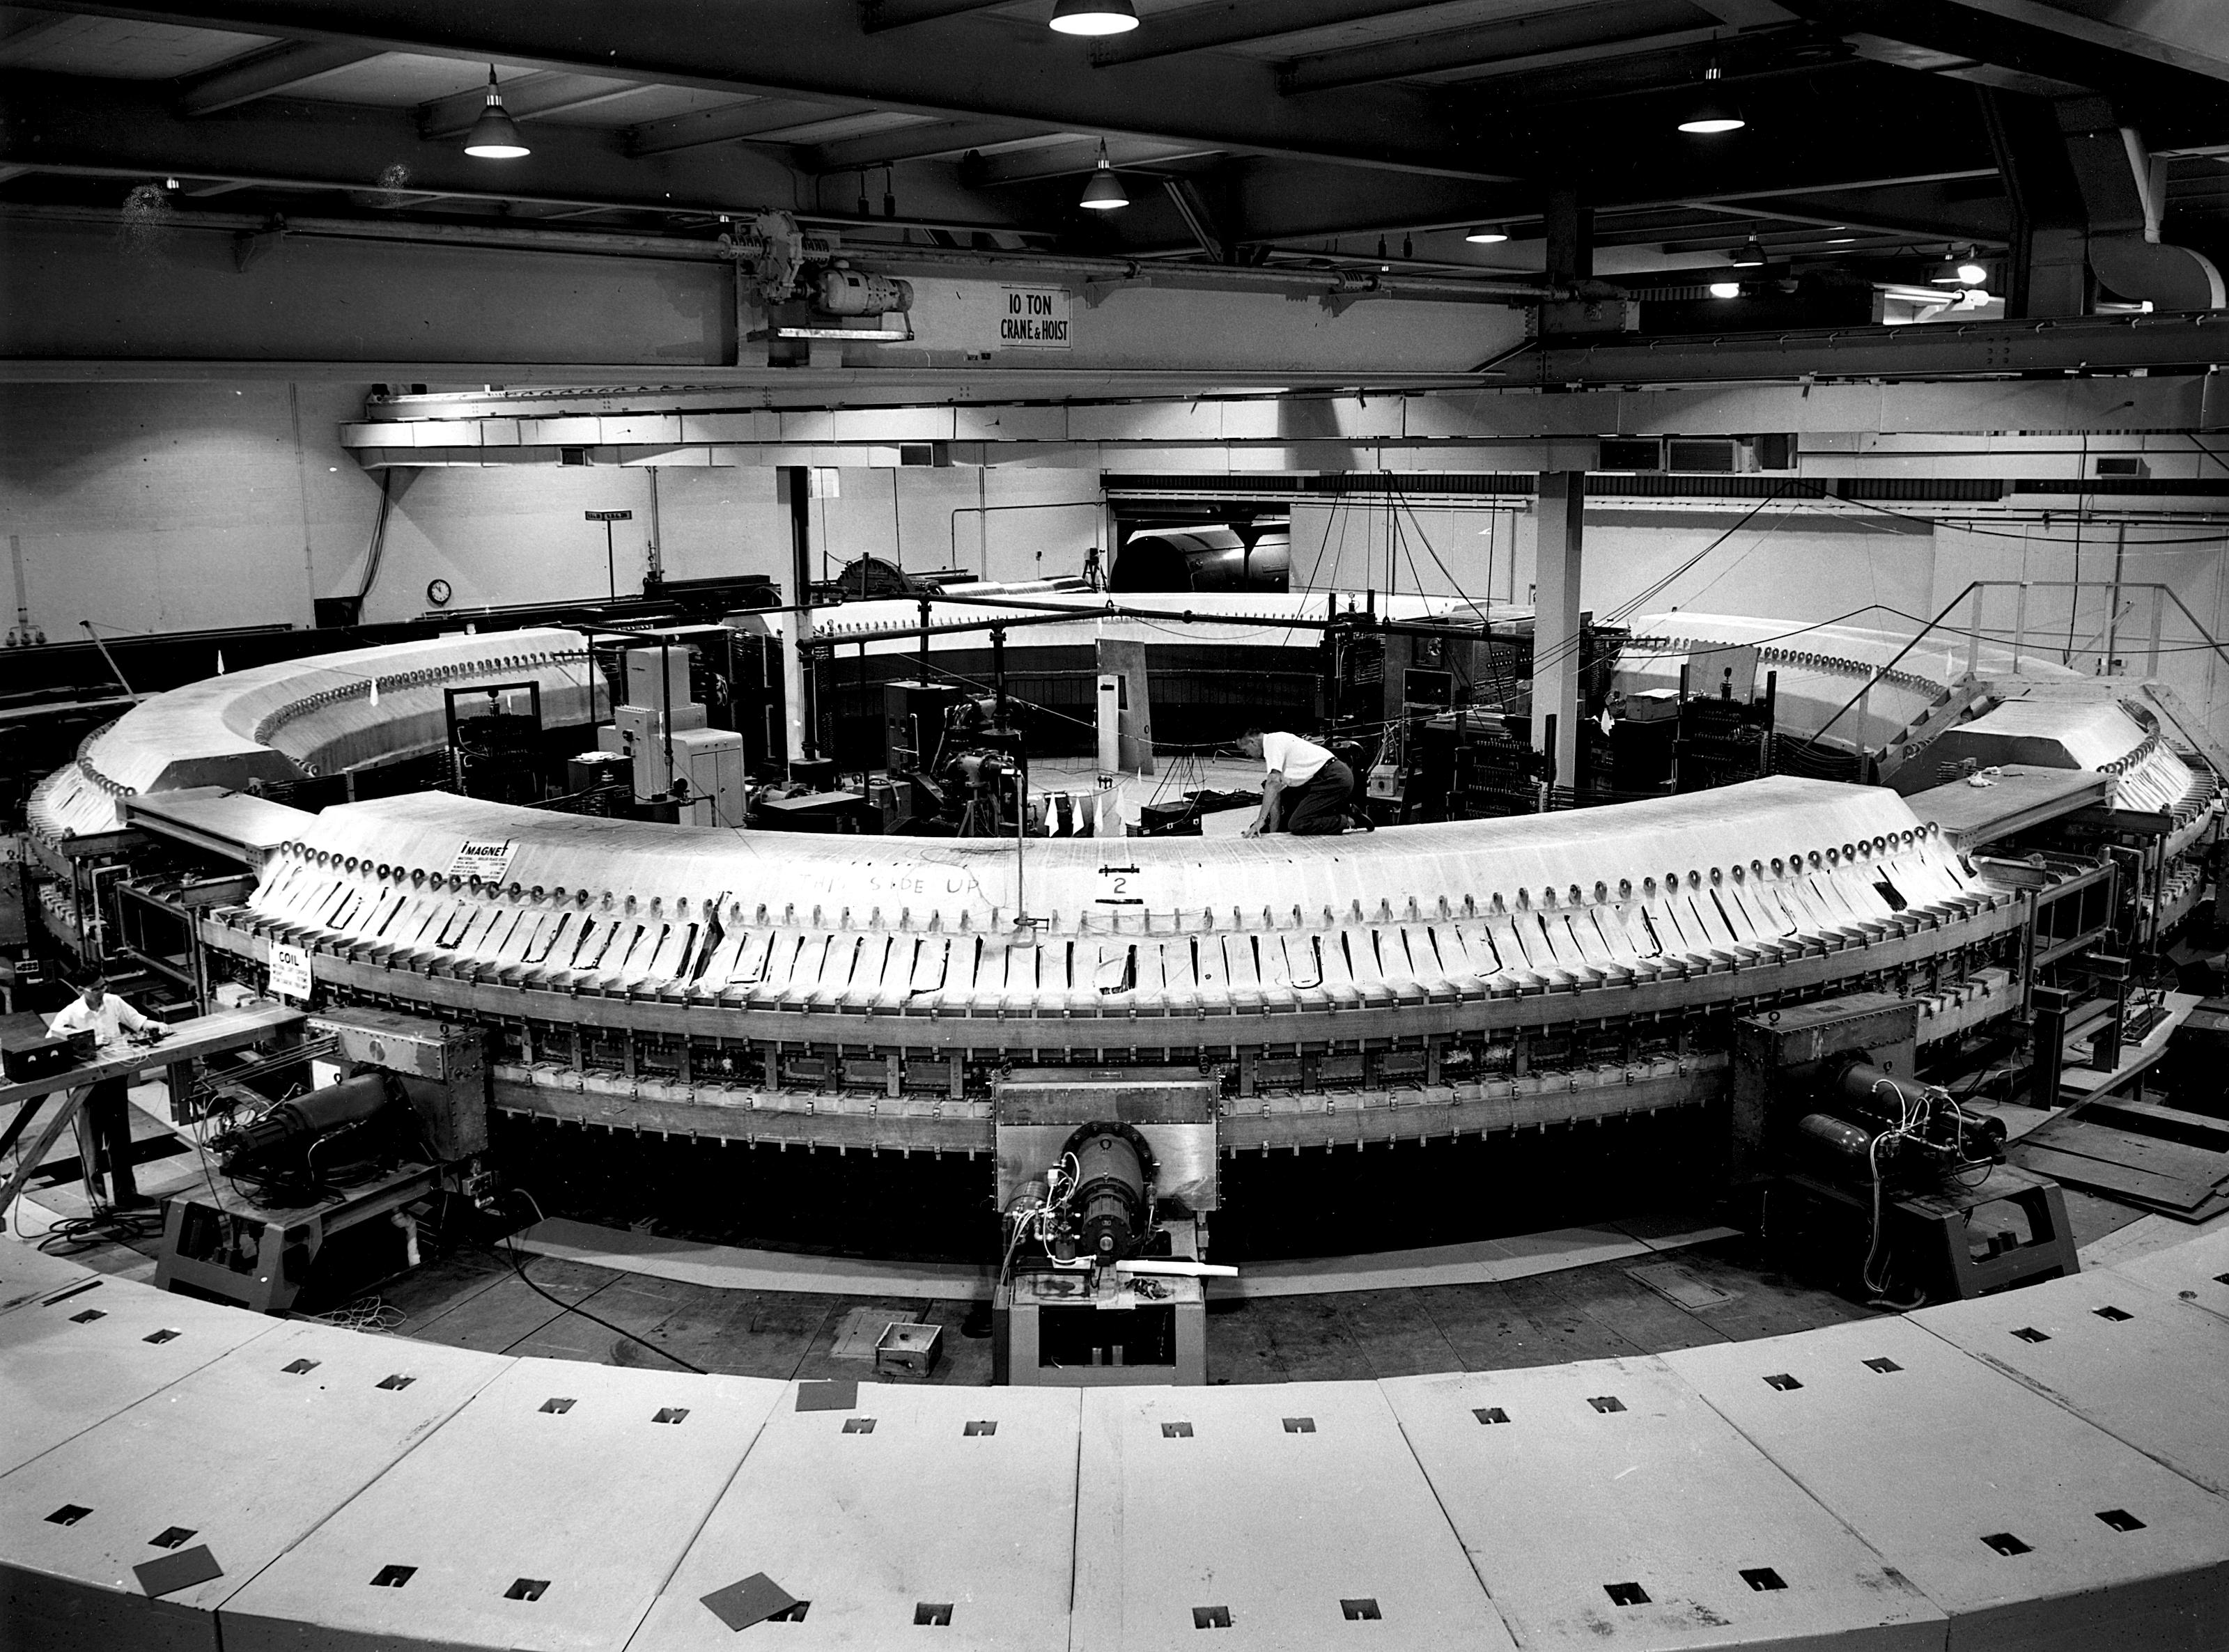
\includegraphics[height=0.6\textheight]{Images/cosmotron.jpg} %Zuschnippeln
            \caption{Das Cosmotron am Brookhaven National Laboratory (1952-1966)}
          \end{center}
        \end{figure}
      \end{column}
      \begin{column}{0.5\textwidth}
        \begin{itemize}
          \item Bau des damals leistungsstärksten Proton-Synchrotron mit Strahlenergien von $\SI{3.3}{\giga\electronvolt}$ im Jahr 1952
          \item Erstmals Produktion von schweren Teilchen der kosmischen Höhenstrahlung möglich
          \item Entdeckung des $K_{L}$ 1956 durch Lande in Nebelkammer
          \item Beobachtung der Paritätsverletzung 1956 durch T.D. Lee und C.N.Yang
          \begin{equation*}
            \tau^{+} \rightarrow \pi^{+} \pi^{+} \pi^{-}
          \end{equation*}
          \begin{equation*}
            \theta^{+} \rightarrow \pi^{+} \pi^{0}
          \end{equation*}
          \item $\tau^{+}$ und $\theta^{+}$ tatsächlich ein Teilchen $K^{+}$, die Zerfälle verletzen also die Paritätserhaltung
        \end{itemize}
      \end{column}
    \end{columns}
  \end{frame}

\subsection{Kaonenmischung}

  \begin{frame}{Long und short? Die Mischung neutraler Kaonen}
    \begin{columns}[onlytextwidth]
      \begin{column}{0.4\textwidth}
        \begin{figure}[ht]
          \feynmandiagram[layered layout, horizontal=a to b, scale=0.9]{
            i1 [particle=\(d\)]
              -- [fermion] a
              -- [photon, edge label=\(W^{-}\)] b
              -- [fermion] f1 [particle=\(\overline s\)],
            i2 [particle=\(\overline s\)]
              -- [anti fermion] c
              -- [photon, edge label'=\(W^{-}\)] d
              -- [anti fermion] f2 [particle=\(d\)],
            { [same layer] a -- [fermion, edge label'=\(u\, c\, t\)] c },
            { [same layer] b -- [anti fermion, edge label=\(u\, c\, t\)] d}
          };
        \end{figure}
        \begin{figure}[ht]
          \feynmandiagram[layered layout, horizontal=a to b, scale=0.9]{
            i1 [particle=\(d\)]
              -- [fermion] a
              -- [fermion, edge label=\(u\, c\, t\)] b
              -- [fermion] f1 [particle=\(\overline s\)],
            i2 [particle=\(\overline s\)]
              -- [anti fermion] c
              -- [anti fermion, edge label'=\(u\, c\, t\)] d
              -- [anti fermion] f2 [particle=\(d\)],
            { [same layer] a -- [photon, edge label'=\(W^{-}\)] c },
            { [same layer] b -- [photon, edge label=\(W^{-}\)] d}
          };
        \end{figure}
      \end{column}
      \begin{column}{0.5\textwidth}
        \begin{itemize}
          \item Die Flavour-Eigenzustände $\ket{K^{0}}$, $\ket{\overline{K^{0}}}$ unterscheiden sich von den CP-Eigenzuständen:
          \begin{equation*}
            \begin{drcases*}
              CP \ket{K^{0}} = \ket{\overline{K^{0}}} \\
              CP \ket{\overline{K^{0}}} = \ket{K^{0}}
            \end{drcases*}
            \rightarrow
            \begin{cases}
              \ket{K_1} = \frac{1}{\sqrt{2}}\left(\ket{K^{0}} + \ket{\overline{K^{0}}} \right) \\
              \ket{K_2} = \frac{1}{\sqrt{2}}\left(\ket{K^{0}} - \ket{\overline{K^{0}}} \right)
            \end{cases}
          \end{equation*}
          \item Dabei ist $\ket{K_1} \approx \ket{K_{S}}$ und $\ket{K_2} \approx \ket{K_{L}}$, mit $\tau(\ket{K_{L}}) \approx 600 \times \tau(\ket{K_{S}})$
          \item $\ket{K_{S}}$ hatben CP = +1 und $\ket{K_{L}}$ habe CP =-1
          \item Unterschied vor allem in Zerfallsmoden:
          \begin{align*}
            \ket{K_{S}} &\rightarrow \pi^{+} \pi^{-} \\ %Mehr Möglichkeiten im Phasenraum
            \ket{K_{L}} &\rightarrow \pi^{+} \pi^{-} \pi^{0} %Eigentlich verboten, s.h. später
          \end{align*}
        \end{itemize}
      \end{column}
    \end{columns}
  \end{frame}

\subsection{Direkte und indirekte CP-Verletzung}

  \begin{frame}{CP-Verletzung}
    \begin{columns}[onlytextwidth]
      \begin{column}{0.4\textwidth}
        \begin{figure}[ht]
          \begin{center}
            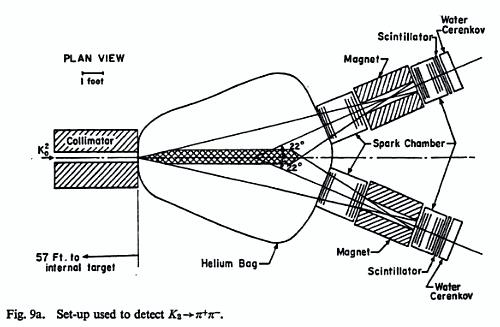
\includegraphics[height=0.6\textheight]{Images/croninfitch.png} %Zuschnippeln
            \caption{Das Cronin-Fitch-Experiment am Brookhaven National Laboratory (1964)}
          \end{center}
        \end{figure}
      \end{column}
      \begin{column}{0.5\textwidth}
        \begin{itemize}
          \item Christenson, Cronin, Fitch und Turlay planen 1964 Experiment am Brookhaven National Laboratory %Collimator => Bündelung de Teilchenstrahlen
          \item $\SI{17}{\metre}$ lange Beamline in der alle $\ket{K_{S}}$ zerfallen sollen und nur noch $\Ket{K_{L}}$ übrig bleiben
          \item Hauptsächlich wird der Winkel $\theta$ zwischen dem $K_{L}^{0}$-Strahl und den Teilchenimpulsen gemessen.
          \item Treffen zwei Teilchen 'gleichzeitig' den Detektor so kann die Summe der Winkel bestimmt werden (aus Spurdetektion)
          \item Diese ist für einen Dreikörperzerfall mit großer Wahrscheinlichkeit $\neq 0$ für Zweikörperzerfälle hingegen mit großer Wahrscheinlichkeit $= 0$
        \end{itemize}
      \end{column}
    \end{columns}
  \end{frame}

  \begin{frame}{Ergebnis}
    \begin{columns}[onlytextwidth]
      \begin{column}{0.4\textwidth}
        \begin{figure}[ht]
          \begin{center}
            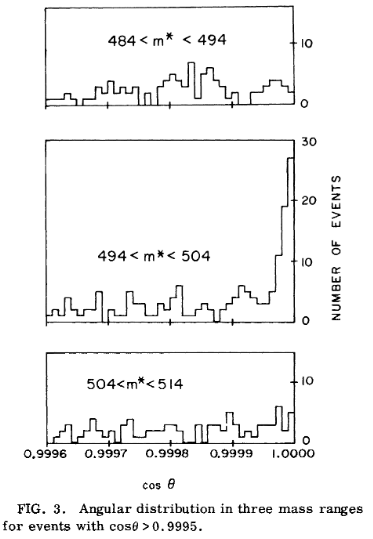
\includegraphics[height=0.8\textheight]{Images/croninfitch_erg.png}
            \caption{Ergebnis der Winkelmessung}
          \end{center}
        \end{figure}
      \end{column}
      \begin{column}{0.5\textwidth}
        Es wurden tatsächlich Zerfälle von
        \begin{align*}
          K_{L} \rightarrow \pi^{+} \pi^{-}
        \end{align*}
        beobachtet.
      \end{column}
    \end{columns}
  \end{frame}

  \begin{frame}{Wie kann das sein?}
    \begin{itemize}
      \item Konsequenz: $\ket{K_{S}}$ und $\Ket{K_{L}}$ keine reinen CP- Zustände, also indirekte CP-Verletzung
    \end{itemize}
    \rightarrow In beiden Zuständen sind kleine Teile des jeweils anderen Zustands enthalten:
    \begin{align*}
      \ket{K_{L}^0} &= \frac{\epsilon \ket{K_1} + \ket{K_2}}{\sqrt{1 + \epsilon^2}} \\
      \ket{K_{S}^0} &= \frac{\ket{K_1} + \epsilon \ket{K_2}}{\sqrt{1 + \epsilon^2}} \\
      |\epsilon| &= (2.229\pm0.010)\times10^{-3}
    \end{align*}
    \begin{itemize}
      \item Die neutralen Kaonenzustände oszillieren über Box-Diagramme in einander über und zerfallen so
      \item Oder direkte CP-Verletzung über Pinguin- Diagramme
      \item Problem: Im Jahre 1964 noch keine Quarks oder der CKM-Mechanismus bekannt
    \end{itemize}
  \end{frame}

  \begin{frame}{Direkte CP- Verletzung}
    \begin{columns}[onlytextwidth]
      \begin{column}{0.4\textwidth}
        \begin{figure}[ht]
          %\feynmandiagram[layered layout, horizontal=a to b, scale=0.9]{
          %  %i2 [particle=\(\overline s\)]
          %  %  -- [anti fermion] c
          %  %  -- [photon, edge label=\(W^{-}\)] d
          %  %  -- [anti fermion] f2 [particle=\(\overline s\)],
          %  %i1 [particle=\(d\)]
          %  %  -- [fermion] a
          %  %  -- [fermion] f1 [particle=\(d\)],
          %  %c -- [fermion, edge label=\(u\, c\, t\)] e
          %  %  -- [fermion, edge label=\(u\, c\, t\)] d,
          %  %e -- [photon, edge label=\(g\, Z\, \gamma\)] a,
          %  i1 [particle=\(\overline s\)]
          %    -- [anti fermion] a
          %    -- [photon, edge label=\(W^{-}\)] b
          %    -- [anti fermion] f1 [particle=\(\overline s\)],
          %  b -- [fermion, quarter left] d -- [fermion, quarter left] a,
          %  c -- [boson] d,
          %  i2 [particle=\(d\)]
          %    -- [fermion] c
          %    -- [fermion] f2 [particle=\(d\)],
          %};
          \begin{tikzpicture}
            \begin{feynman}
              \vertex(a1){\(\overline s\)};
              \vertex[right=2cm of a1] (a2);
              \vertex[right=0.5cm of a2] (a3);
              \vertex[right=0.5cm of a3] (a4);
              \vertex[right=2cm of a4] (a5){\(\overline d\)};

              \vertex[below=2cm of a1] (b1){\(d\)};
              \vertex[below=2cm of a5] (b2){\(d\)};

              \vertex[below=1.5em of a5] (c1){\(u\)};
              \vertex[above=1.5em of b2] (c3){\(\overline u\)};
              \vertex at ($(c1)!0.5!(c3)- (1cm, 0)$) (c2);

              \diagram* {
                {[edges=fermion]
                  (a5)-- (a4)-- (a3)-- (a2)-- (a1),
                },
                (b1)-- [fermion] (b2),
                (c3)-- [fermion,out=180,in=-60] (c2)-- [fermion,out=60,in=180] (c1),
                (a3)-- [gluon, bend right, edge label'=\(g\, Z\, \gamma\)] (c2),
                (a4)-- [boson,out=90,in=90,looseness=2.0,edge label'=\(W\)] (a2)
              };

              \draw[decoration={brace}, decorate] (b1.south west)-- (a1.north west)
                node[pos=0.5, left] {  \(K^{0}\)};
              \draw[decoration={brace}, decorate] (a5.north east)-- (c1.south east)
                node[pos=0.5, right] {  \(\pi^{+}\)};
              \draw[decoration={brace}, decorate] (c3.north east)-- (b2.south east)
                node[pos=0.5, right] {  \(\pi^{-}\)};
            \end{feynman}
          \end{tikzpicture}
          \caption{Pinguindiagramm des CP-verletzenden, neutralen Kaonenzerfalls}
        \end{figure}
      \end{column}
      \begin{column}{0.5\textwidth}
        \begin{itemize}
          \item Direkte CP-Verletzung würde eine CP-Verletzung innerhalb des Zerfalls ohne vorherige Mischung der Kaonen voraussetzen
          \item Messung der partiellen Zerfallsbreiten von:
          \begin{align*}
            K_{L}^0 &\rightarrow \pi^+ \pi^- \\
            K_{L}^0 &\rightarrow \pi^0 \pi^0 \\
            K_{S}^0 &\rightarrow \pi^+ \pi^- \\
            K_{S}^0 &\rightarrow \pi^0 \pi^0
          \end{align*}
          \item Es muss das Verhältnis gebildet werden, da sowohl Anteile der direkten als auch der indirekten Verletzung eine Rolle spielen müssen
        \end{itemize}
      \end{column}
    \end{columns}
  \end{frame}

%\section{Kaptel 2}
  %\begin{frame}{Folie 2.1}
    %Text
  %\end{frame}

\end{document}
